% 这是中国科学院大学计算机科学与技术专业《计算机组成原理(研讨课)》使用的实验报告 Latex 模板
% 本模板与 2024 年 2 月 Jun-xiong Ji 完成, 更改自由 Shing-Ho Lin 和 Jun-Xiong Ji 于 2022 年 9 月共同完成的基础物理实验模板
% 如有任何问题, 请联系: jijunxoing21@mails.ucas.ac.cn
% This is the LaTeX template for report of Experiment of Computer Organization and Design courses, based on its provided Word template. 
% This template is completed on Febrary 2024, based on the joint collabration of Shing-Ho Lin and Junxiong Ji in September 2022. 
% Adding numerous pictures and equations leads to unsatisfying experience in Word. Therefore LaTeX is better. 
% Feel free to contact me via: jijunxoing21@mails.ucas.ac.cn

\documentclass[11pt]{article}

\usepackage[a4paper]{geometry}
\geometry{left=2.0cm,right=2.0cm,top=2.5cm,bottom=2.5cm}

\usepackage{ctex} % 支持中文的LaTeX宏包
\usepackage{amsmath,amsfonts,graphicx,subfigure,amssymb,bm,amsthm,mathrsfs,mathtools,breqn} % 数学公式和符号的宏包集合
\usepackage{algorithm,algorithmicx} % 算法和伪代码
\usepackage[noend]{algpseudocode} % 算法和伪代码
\usepackage{fancyhdr} % 自定义页眉页脚
\usepackage[framemethod=TikZ]{mdframed} % 创建带边框的框架
\usepackage{fontspec} % 字体设置
\usepackage{adjustbox} % 调整盒子大小
\usepackage{fontsize} % 设置字体大小
\usepackage{tikz,xcolor} % 绘制图形和使用颜色
\usepackage{multicol} % 多栏排版
\usepackage{multirow} % 表格中合并单元格
\usepackage{pdfpages} % 插入PDF文件
\usepackage{listings} % 在文档中插入源代码
\usepackage{wrapfig} % 文字绕排图片
\usepackage{bigstrut,multirow,rotating} % 支持在表格中使用特殊命令
\usepackage{booktabs} % 创建美观的表格
\usepackage{circuitikz} % 绘制电路图
\usepackage{zhnumber} % 中文序号(用于标题)
\usepackage{tabularx} % 表格折行

\definecolor{dkgreen}{rgb}{0,0.6,0}
\definecolor{gray}{rgb}{0.5,0.5,0.5}
\definecolor{mauve}{rgb}{0.58,0,0.82}
\lstset{
  frame=tb,
  aboveskip=3mm,
  belowskip=3mm,
  showstringspaces=false,
  columns=flexible,
  framerule=1pt,
  rulecolor=\color{gray!35},
  backgroundcolor=\color{gray!5},
  basicstyle={\small\ttfamily},
  numbers=none,
  numberstyle=\tiny\color{gray},
  keywordstyle=\color{blue},
  commentstyle=\color{dkgreen},
  stringstyle=\color{mauve},
  breaklines=true,
  breakatwhitespace=true,
  tabsize=3,
}

% 轻松引用, 可以用\cref{}指令直接引用, 自动加前缀. 
% 例: 图片label为fig:1
% \cref{fig:1} => Figure.1
% \ref{fig:1}  => 1
\usepackage[capitalize]{cleveref}
% \crefname{section}{Sec.}{Secs.}
\Crefname{section}{Section}{Sections}
\Crefname{table}{Table}{Tables}
\crefname{table}{Table.}{Tabs.}

% \setmainfont{Palatino Linotype.ttf}
% \setCJKmainfont{SimHei.ttf}
% \setCJKsansfont{Songti.ttf}
% \setCJKmonofont{SimSun.ttf}
\punctstyle{kaiming}
% 偏好的几个字体, 可以根据需要自行加入字体ttf文件并调用

\renewcommand{\emph}[1]{\begin{kaishu}#1\end{kaishu}}

% 对 section 等环境的序号使用中文
\renewcommand \thesection{\zhnum{section}、}
\renewcommand \thesubsection{\arabic{section}}


%%%%%%%%%%%%%%%%%%%%%%%%%%%
%改这里可以修改实验报告表头的信息
\newcommand{\name}{艾华春, 李霄宇, 王敬华}
\newcommand{\studentNum}{2022K8009916011,2022K8009929029,2022K8009925009}
\newcommand{\major}{计算机科学与技术}
\newcommand{\labNum}{3}
\newcommand{\labName}{在流水线中添加普通用户态指令}
%%%%%%%%%%%%%%%%%%%%%%%%%%%

\begin{document}

\begin{center}
  \LARGE \bf 中国科学院大学 \\《计算机体系结构基础(研讨课)》实验报告
\end{center}

\begin{center}
  \emph{姓名} \underline{\makebox[10em][c]{\name}} \\
  % 如果名字比较长, 可以修改box的长度"8em"为其他值
  \emph{学号} \underline{\makebox[30em][c]{\studentNum}}\\
  % \emph{专业} \underline{\makebox[15em][c]{\major}}\\
  \emph{实验项目编号} \underline{\makebox[3em][c]{\labNum}}
  \emph{实验名称} \underline{\makebox[30em][c]{\labName}}\\
\end{center}

% \begin{center}
%   \begin{tabularx}{\textwidth}{|lX|}
%     \hline
%     注1: & 撰写此 Word 格式实验报告后以 PDF 格式保存 SERVE CloudIDE 的 \texttt{/home/serve-ide/ cod-lab/reports} 目录下(注意:reports 全部小写)。文件命名规则:\texttt{prjN.pdf},其中 \texttt{prj} 和后缀名 \texttt{pdf} 为小写,\texttt{N} 为1至4的阿拉伯数字。例如:\texttt{prj1.pdf}。PDF 文件大小应控制在 5MB 以内。此外,实验项目5包含多个选做内容,每个选做实验应提交各自的实验报告文件,文件命名规则:\texttt{prj5-projectname.pdf},其中``-''为英文标点符号的短横线。文件命名举例:\texttt{prj5-dma.pdf}。具体要求详见实验项目5讲义。 \\

%     注2: & 使用\texttt{git add}及\texttt{git commit}命令将实验报告\texttt{PDF}文件添加到本地仓库master分支,并通过\texttt{git push}推送到实验课SERVE GitLab远程仓库master分支(具体命令详见实验报告)。 \\

%     注3: & 实验报告模板下列条目仅供参考,可包含但不限定如下内容。实验报告中无需重复描述讲义中的实验流程。\\
%     \hline
%   \end{tabularx}
% \end{center}

  

\section{逻辑电路结构与仿真波形的截图及说明}
\noindent
$\bullet$
\textbf{算数逻辑运算和乘除类运算指令添加}。
\begin{enumerate}
  \item 首先添加算数逻辑运算数据通路
  
  首先对逻辑信号进行译码操作,得到各个指令的信号(ID阶段)

  \begin{lstlisting}[language=verilog]
    assign inst_slti   = op_31_26_d[6'h00] & op_25_22_d[4'h8];
    assign inst_sltui  = op_31_26_d[6'h00] & op_25_22_d[4'h9];
    assign inst_andi   = op_31_26_d[6'h00] & op_25_22_d[4'hd];
    assign inst_ori    = op_31_26_d[6'h00] & op_25_22_d[4'he];
    assign inst_xori   = op_31_26_d[6'h00] & op_25_22_d[4'hf];
    assign inst_sll_w  = op_31_26_d[6'h00] & op_25_22_d[4'h0] & op_21_20_d[2'h1] & op_19_15_d[5'h0e];
    assign inst_srl_w  = op_31_26_d[6'h00] & op_25_22_d[4'h0] & op_21_20_d[2'h1] & op_19_15_d[5'h0f];
    assign inst_sra_w  = op_31_26_d[6'h00] & op_25_22_d[4'h0] & op_21_20_d[2'h1] & op_19_15_d[5'h10];
    assign inst_pcaddul2i = op_31_26_d[6'h07] & ~id_inst[25];
    assign inst_mul_w  = op_31_26_d[6'h00] & op_25_22_d[4'h0] & op_21_20_d[2'h1] & op_19_15_d[5'h18];
    assign inst_mulh_w = op_31_26_d[6'h00] & op_25_22_d[4'h0] & op_21_20_d[2'h1] & op_19_15_d[5'h19];
    assign inst_mulh_wu= op_31_26_d[6'h00] & op_25_22_d[4'h0] & op_21_20_d[2'h1] & op_19_15_d[5'h1a];
    assign inst_div_w  = op_31_26_d[6'h00] & op_25_22_d[4'h0] & op_21_20_d[2'h2] & op_19_15_d[5'h00];
    assign inst_mod_w  = op_31_26_d[6'h00] & op_25_22_d[4'h0] & op_21_20_d[2'h2] & op_19_15_d[5'h01];
    assign inst_div_wu = op_31_26_d[6'h00] & op_25_22_d[4'h0] & op_21_20_d[2'h2] & op_19_15_d[5'h02];
    assign inst_mod_wu = op_31_26_d[6'h00] & op_25_22_d[4'h0] & op_21_20_d[2'h2] & op_19_15_d[5'h03];
  \end{lstlisting}

  然后根据各条指令的需求,分别对应各条指令需要的alu操作数
  \begin{lstlisting}[language=verilog]
    assign id_alu_op[ 0] = inst_add_w | inst_addi_w | inst_ld_w | inst_st_w  | inst_ld_b | inst_ld_h | inst_ld_bu | inst_ld_hu | inst_st_b | inst_st_h
                        | inst_jirl | inst_bl | inst_pcaddul2i;
    assign id_alu_op[ 1] = inst_sub_w;
    assign id_alu_op[ 2] = inst_slt | inst_slti;
    assign id_alu_op[ 3] = inst_sltu | inst_sltui;
    assign id_alu_op[ 4] = inst_and | inst_andi;
    assign id_alu_op[ 5] = inst_nor;
    assign id_alu_op[ 6] = inst_or | inst_ori;
    assign id_alu_op[ 7] = inst_xor | inst_xori;
    assign id_alu_op[ 8] = inst_slli_w | inst_sll_w;
    assign id_alu_op[ 9] = inst_srli_w | inst_srl_w;
    assign id_alu_op[10] = inst_srai_w | inst_sra_w;
    assign id_alu_op[11] = inst_lu12i_w;
    assign id_alu_op[12] = inst_mul_w ;
    assign id_alu_op[13] = inst_mulh_w;
    assign id_alu_op[14] = inst_mulh_wu;
    assign id_alu_op[15] = inst_div_w;
    assign id_alu_op[16] = inst_div_wu;
    assign id_alu_op[17] = inst_mod_w;
    assign id_alu_op[18] = inst_mod_wu;
  \end{lstlisting}

  注意,此处对alu进行乘除法拓展,已经扩展为19位数,其中alu[18:12]为乘除法运算的alu操作码

  接着,还需要更新ID模块中对alu源操作数的选择,并且为了前递处理流水线冲突,还需要更新指令使用寄存器1或(和)寄存器2的信号
  \begin{lstlisting}[language=verilog]
    assign id_src1_is_pc    = inst_jirl | inst_bl | inst_pcaddul2i;
    assign id_src2_is_imm   = inst_slli_w |
                              inst_srli_w |
                              inst_srai_w |
                              inst_addi_w |
                              inst_ld_w   |
                              inst_st_w   |
                              inst_lu12i_w|
                              inst_jirl   |
                              inst_bl     |
                              inst_pcaddul2i|
                              inst_andi   |
                              inst_ori    |
                              inst_xori   |
                              inst_slti   |
                              inst_sltui  |
                              inst_ld_b   |
                              inst_ld_h   |
                              inst_ld_bu  |
                              inst_ld_hu  |
                              inst_st_b   |
                              inst_st_h;
  \end{lstlisting}
  \begin{lstlisting}[language=verilog]
    assign need_r1         = ~inst_b & ~inst_bl & ~inst_lu12i_w & ~inst_pcaddul2i;//需要使用(读)源寄存器1(rj)的指令
    assign need_r2         =  inst_add_w | inst_sub_w | inst_slt | inst_sltu | inst_and | inst_or | inst_nor | inst_xor
                              | inst_beq | inst_bne | inst_blt | inst_bge | inst_bltu | inst_bgeu                           //添加blt等指令
                              | inst_st_w | inst_sll_w| inst_srl_w | inst_sra_w | inst_mul_w 
                              | inst_mulh_w | inst_mulh_wu | inst_mod_w | inst_mod_wu | inst_div_w |inst_div_wu
                              | inst_st_b | inst_st_h;
                              //需要使用(读)源寄存器2(rk/rd)的指令
  \end{lstlisting}

  最后,只需要更新各条指令需要的立即数格式,并且修改各个模块之间通信的总线位宽即可
  \begin{lstlisting}[language=verilog]
    assign need_ui5   =  inst_slli_w | inst_srli_w | inst_srai_w;
    assign need_si12  =  inst_addi_w | inst_ld_w | inst_st_w | inst_slti | inst_sltui 
                        | inst_ld_b | inst_ld_h | inst_ld_bu | inst_ld_hu | inst_st_b | inst_st_h;
    assign need_si16  =  inst_jirl | inst_beq | inst_bne | inst_blt | inst_bge | inst_bltu | inst_bgeu;     //添加blt等指令
    assign need_si20  =  inst_lu12i_w | inst_pcaddul2i;
    assign need_si26  =  inst_b | inst_bl;
    assign need_ui12  =  inst_andi   | inst_ori | inst_xori ;
    assign src2_is_4  =  inst_jirl | inst_bl;    
  \end{lstlisting}

  \item 实现对alu模块的修改,使其能够实现乘除法运算
  
  首先,在alu中引入节拍clk,并且引入complete信号用于标识运算结束,
  这样可以使alu运算在节拍上与流水线一致,并且一个节拍运算完成不了的情
  况下(切分成两级流水结构的乘法器或者除法器模块),可以进行流水线阻塞来进行等待。
  \begin{lstlisting}[language=verilog]
    module alu(
      input  wire        clk,
      input  wire        resetn,
      // input  wire [11:0] alu_op,
      input  wire [18:0] alu_op,
      input  wire [31:0] alu_src1,
      input  wire [31:0] alu_src2,
      output wire [31:0] alu_result,
      output wire        complete
    );
    assign complete = ~resetn | div_complete & div_en | mul_complete & mul_en | ~div_en & ~mul_en;
  \end{lstlisting}

  在EX阶段实例化alu,并且实现一个节拍运算完成不了的情况(切分成两级流水结构的乘法器或者除法器模块),可以进行
  流水线阻塞来进行等待。这里要尤其注意接口位宽的定义,防止疏忽出错。
  \begin{lstlisting}[language=verilog]
    alu u_alu(
      .clk            (clk       ),
      .resetn         (resetn    ),
      .alu_op         (ex_alu_op    ),
      .alu_src1       (ex_alu_src1  ),
      .alu_src2       (ex_alu_src2  ),
      .alu_result     (ex_alu_result),
      .complete       (alu_complete)
  );
  assign ex_ready_go      = alu_complete;//等待alu完成运算
  \end{lstlisting}

  接着,在alu中实现乘法器模块和除法器模块的实例化,其中的使能信号对应如下:
  \begin{lstlisting}[language=verilog]
    Wallace_Mul u_mul(
    .mul_clk(clk),
    .resetn(resetn),
    .mul_signed(op_mulh|op_mul),
    .A(alu_src1),
    .B(alu_src2),
    .result(mul_result)
);

    Div u_div(
    .div_clk(clk),
    .resetn(resetn),
    .div(div_en),
    .div_signed(op_mod | op_div),
    .x(alu_src1),
    .y(alu_src2),
    .s(div_result),
    .r(mod_result),
    .complete(div_complete)
);
    assign mul_en = op_mul | op_mulh | op_mulhu;
    assign div_en = op_mod | op_modu | op_div | op_divu;
  \end{lstlisting}

  最后对result的选择器进行更新即可
  \begin{lstlisting}[language=verilog]
    assign alu_result = ({32{op_add|op_sub}} & add_sub_result)
                  | ({32{op_slt       }} & slt_result)
                  | ({32{op_sltu      }} & sltu_result)
                  | ({32{op_and       }} & and_result)
                  | ({32{op_nor       }} & nor_result)
                  | ({32{op_or        }} & or_result)
                  | ({32{op_xor       }} & xor_result)
                  | ({32{op_lui       }} & lui_result)
                  | ({32{op_sll       }} & sll_result)
                  | ({32{op_srl|op_sra}} & sr_result)
                  | ({32{op_mod|op_modu}} & mod_result)
                  | ({32{op_div|op_divu}} & div_result)
                  | ({32{op_mul       }} & mul_result[31:0])
                  | ({32{op_mulh|op_mulhu}} & mul_result[63:32]);

  \end{lstlisting}

  \item 实现乘法器和除法器
  
  乘法器构建的华莱士树一共有六层,每层华莱士树中的加法器是并行的。故考虑在3~4层加法器
  中做流水线分割,使得两级流水线的操作时长差异较小。
  对于除法器就简单的多了,采用恢复余数迭代除法器,当counter == 6'd33的时候发送运算完成信号。\par


  注:实际上乘法器和除法器的具体内容并不是我本人设计的,而是参考了互联网上的一些博客/github来源内容以及
  chatgpt进行的代码修改以适应本实验的使用环境。这样做的初衷是作为调用 Xilinx IP核的一个平替(因为此次实验本来就
  允许调用Xilinx IP),本来也没有想要通过这个获得额外的加分,只是想要简单了解一下乘除法的底层运算机制。

\end{enumerate}

\noindent
$\bullet$
\textbf{转移指令添加}。
\begin{enumerate}
    \item 首先添加无符号数和有符号数小于比较结果的数据通路

    无符号数比较直接使用<进行判断,有符号数比较先将操作数转换成signed在进行比较。

    \begin{lstlisting}[language=verilog]
    assign rj_ltu_rd = (rj_value < rkd_value);                                   //无符号数比较:GR[rj]小于GR[rd]                          
    assign rj_lt_rd = ($signed(rj_value) < $signed(rkd_value));       //有符号数比较:GR[rj]小于GR[rd]
    \end{lstlisting}

    \item 再据此补全跳转条件

    blt和bltu可直接使用rj\_ltu\_rd和rj\_lt\_rd作为跳转条件,bge和bgeu则直接将二者取反即可。

    \begin{lstlisting}[language=verilog]
    assign br_taken = (inst_beq  &&  rj_eq_rd
                    || inst_bne  && !rj_eq_rd
                    || inst_blt  &&  rj_lt_rd                                 //添加blt等指令的跳转条件
                    || inst_bge  && !rj_lt_rd
                    || inst_bltu &&  rj_ltu_rd
                    || inst_bgeu &&  !rj_ltu_rd
                    || inst_jirl
                    || inst_bl
                    || inst_b
                    ) && id_valid;
    \end{lstlisting}

    \item 跳转地址复用

    新添加的四个跳转指令跳转地址可直接复用beq等指令的控制逻辑。

    \begin{lstlisting}[language=verilog]
    assign br_target = (inst_beq || inst_bne || inst_blt || inst_bltu || inst_bge || inst_bgeu || inst_bl || inst_b) ? (id_pc + br_offs) :
        /*inst_jirl*/ (rj_value + jirl_offs);        //添加blt等指令的跳转地址:与bne,beq相同
    \end{lstlisting}
\end{enumerate}

\noindent
$\bullet$
\textbf{访存指令添加}。
\begin{enumerate}
  \item 添加访存操作类型的数据通路
  
  在ID(译码)阶段添加判断当前的load 或 store操作的类型,包括是否无符号扩展,数据的位宽。并将相应的信号沿着流水级传递到MEM(访存)阶段。

  \begin{lstlisting}[language=verilog]
    assign id_op_st_ld_b      = op_25_22[1:0] == 2'd0;    // 位宽为1 byte
    assign id_op_st_ld_h      = op_25_22[1:0] == 2'd1;    // 位宽为2 byte
    assign id_op_st_ld_u      = op_25_22[3];              // 无符号数扩展
  \end{lstlisting}
\item 添加从EX到MEM访存地址最低两位传递数据通路

  在EX到MEM的传递的数据中添加访存地址的最低两个bit,使得MEM阶段可以获取到从sram中取出来1字节的数据内部的偏移。

  \item 在load操作的结果处添加多路选择器(在访存流水级)
  
  首先,通过操作的数据位宽和访存地址来选择出从sram中输出的的数据的有效部分。
  \begin{lstlisting}[language=verilog]
    // mem_data_sram_addr[2] 是上一小节中传递过到mem级的访存地址后两位
    assign mem_word_result =    data_sram_rdata;   // ld.w 的有效部分
    assign mem_half_result =    mem_data_sram_addr[1] ? data_sram_rdata[31:16]
                                : data_sram_rdata[15:0];    // ld.h 的有效部分
    assign mem_byte_result =    ({8{mem_data_sram_addr[1:0] == 2'd0}} & data_sram_rdata[7:0])
                                |({8{mem_data_sram_addr[1:0] == 2'd1}} & data_sram_rdata[15:8])
                                |({8{mem_data_sram_addr[1:0] == 2'd2}} & data_sram_rdata[23:16])
                                |({8{mem_data_sram_addr[1:0] == 2'd3}} & data_sram_rdata[31:24]);
                                // ld.b 的有效部分

  \end{lstlisting}

  然后根据有符号扩展还是无符号数扩展,对结果进行扩展,最终得到可以写入目的寄存器(rd)的结果\verb|mem_result|。
  \begin{lstlisting}[language=verilog]
    // mem_op_st_ld_b, mem_op_st_ld_h 分别表示数据位宽为1byte和2byte
    // mem_op_st_ld_u 表示数据进行无符号数扩展(即0扩展)
    // ~mem_op_st_ld_u & mem_byte_result[7]  或~mem_op_st_ld_u & mem_half_result[15] 表示符号位
    assign mem_result 
    = mem_op_st_ld_b ? ({{24{~mem_op_st_ld_u & mem_byte_result[7]}}, mem_byte_result[7:0]}):       
      mem_op_st_ld_h ? ({{16{~mem_op_st_ld_u & mem_half_result[15]}}, mem_half_result[15:0]}) :
      mem_word_result;
  \end{lstlisting}

  \item 在store操作中传递给\verb|data_sram|的信号处添加选择器
  
  首先,根据访存的位宽和地址,通过多路选择和移位操作确定字节使能信号。
  \begin{lstlisting}[language=verilog]
    // 字节使能
    // st.b 时,根据访存地址的最低两位进行移位操作。有四种不同情况
    // st.h 时,根据访存地址的最低两位添加二选以选择器。有两种不同情况
    assign ex_sram_we = ex_op_st_ld_b ? (4'b0001 << ex_data_sram_addr[1:0]) :           // st.b
                      ex_op_st_ld_h ? (ex_data_sram_addr[1] ? 4'b1100 : 4'b0011) :    // st.h
                      4'b1111;                                    // st.w
  \end{lstlisting}
  确定字节使能后,生成写入数据。不需要将数据进行移动,而是仅仅根据数据长度,对有效部分进行复制连接操作,
  确保数据在写入时能拿到有效的数据。
\begin{lstlisting}[language=verilog]
  //生成写入数据
  //对有效部分进行复制连接操作
  assign data_sram_wdata  =    ex_op_st_ld_b ? {4{ex_rkd_value[7:0]}}:
                              ex_op_st_ld_h ? {2{ex_rkd_value[15:0]}}:
                              ex_rkd_value[31:0];
\end{lstlisting}
\end{enumerate}




\vspace{1ex}

\section{实验过程中遇到的问题、对问题的思考过程及解决方法(比如RTL代码中出现的逻辑bug,逻辑仿真和FPGA调试过程中的难点等)}

\noindent
$\bullet$
\textbf{data_sram写使能bug}。
一开始时有符号数的比较条件尝试不使用类型转换的方法去写一个有符号数比较器。
\begin{lstlisting}[language=verilog]
 assign signed_cmp = rj_value[31] ? (rkd_value[31] ? rj_gt_rd : 1'b1) :         
                                       (rkd_value[31] ? 1'b1 : rj_lt_rd);       //有符号数比较:GR[rj]小于GR[rd]
\end{lstlisting}

仿真时发现跳转出错,再波形图中擦好看发现signed\_cmp变量出现问题,仔细查看发现GR[rj]为负而GR[rd]为正时以及GR[rj]为正而GR[rd]为负时赋值反了,于是干脆就直接改用类型转换的方法做有符号数比较了。
\begin{lstlisting}
assign rj_lt_rd = ($signed(rj_value) < $signed(rkd_value));       //有符号数比较:GR[rj]小于GR[rd]
\end{lstlisting}
\vspace{1ex}

\noindent
$\bullet$
\textbf{data_sram写使能bug}。
在仿真中,在load指令中,写入寄存器的结果与标准结果不一致。

然后在波形图中查看从sram直接返回的数据,发现同样与标准结果不一致,于是排除是新添加的load多路选择器的问题。

进而在反汇编代码中,发现在load指令前,有一条store指令,地址相同。于是在波形图中查看相关波形,发现该指令ex阶段的sram写使能没有拉高,再回溯到id阶段,
发现是mem写使能中,不同种类的load之间的逻辑连接错写成与,导致不能向sram写入数据。

\begin{lstlisting}[language=verilog]
//  assign id_mem_we        = inst_st_w & inst_st_b & inst_st_h & id_valid;  
assign id_mem_we        = (inst_st_w | inst_st_b | inst_st_h) & id_valid;  
\end{lstlisting}
\vspace{1ex}

\noindent
$\bullet$
\textbf{模块之间通信位宽定义错误}。
错误的现象表现为debug_pc信号一直为0,虽然一直在运行,最后只能暂停仿真。
观察仿真的波形可以发现一些信号的值为高阻态Z,这说明一些信号在运行的时候丢失或者没有进行
定义,如图所示。
\begin{figure}[h]
  \centering
  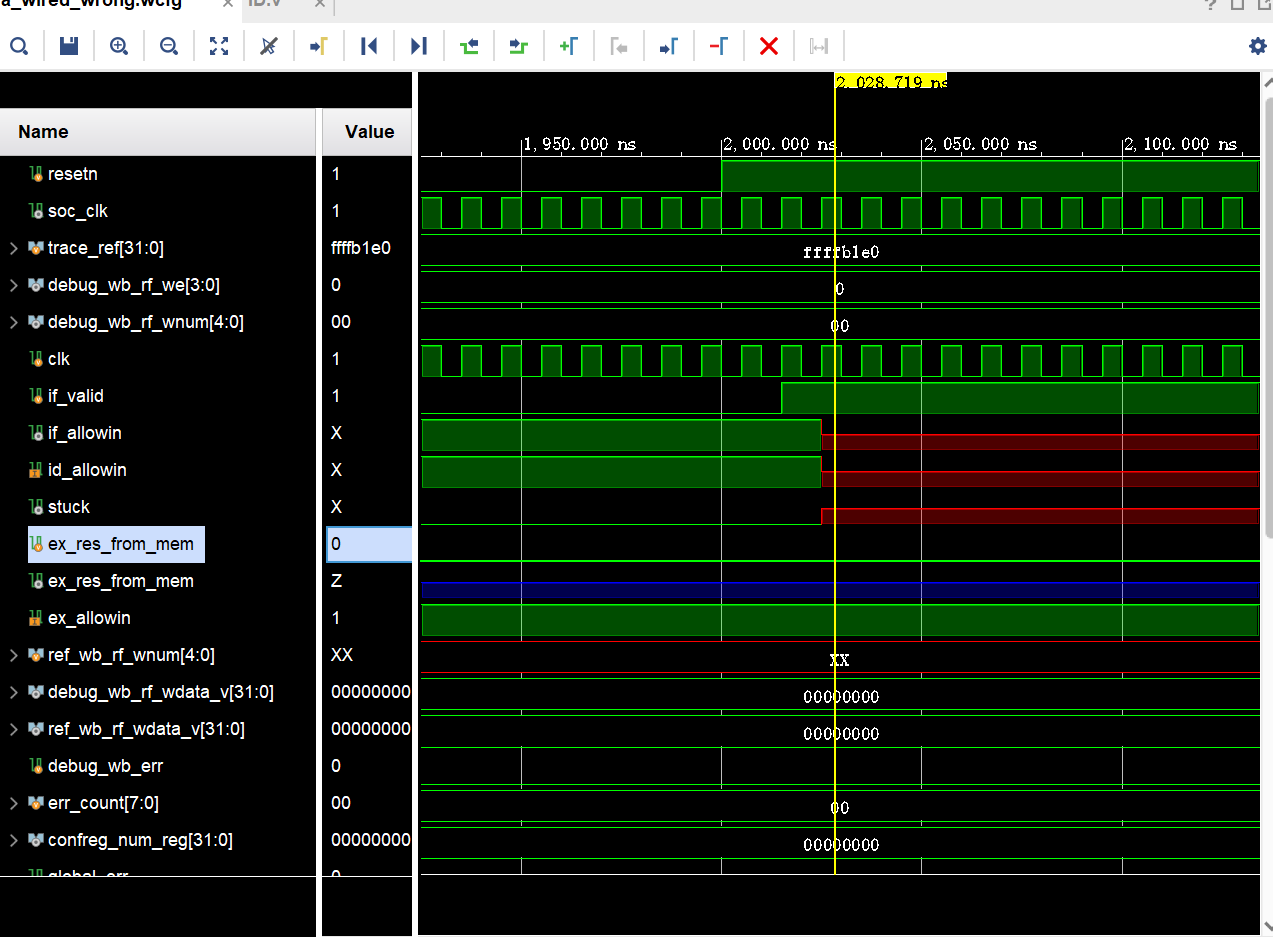
\includegraphics[width=10cm]{fig/1.png}
\end{figure}
追根溯源发现是exe阶段的信号总线位宽定义出错,导致不能收到返回数据,修改之后即可正常。

\vspace{1ex}

\noindent
$\bullet$
\textbf{alu乘法器模块嵌入错误}。
报错如下。
\begin{figure}[H]
  \centering
  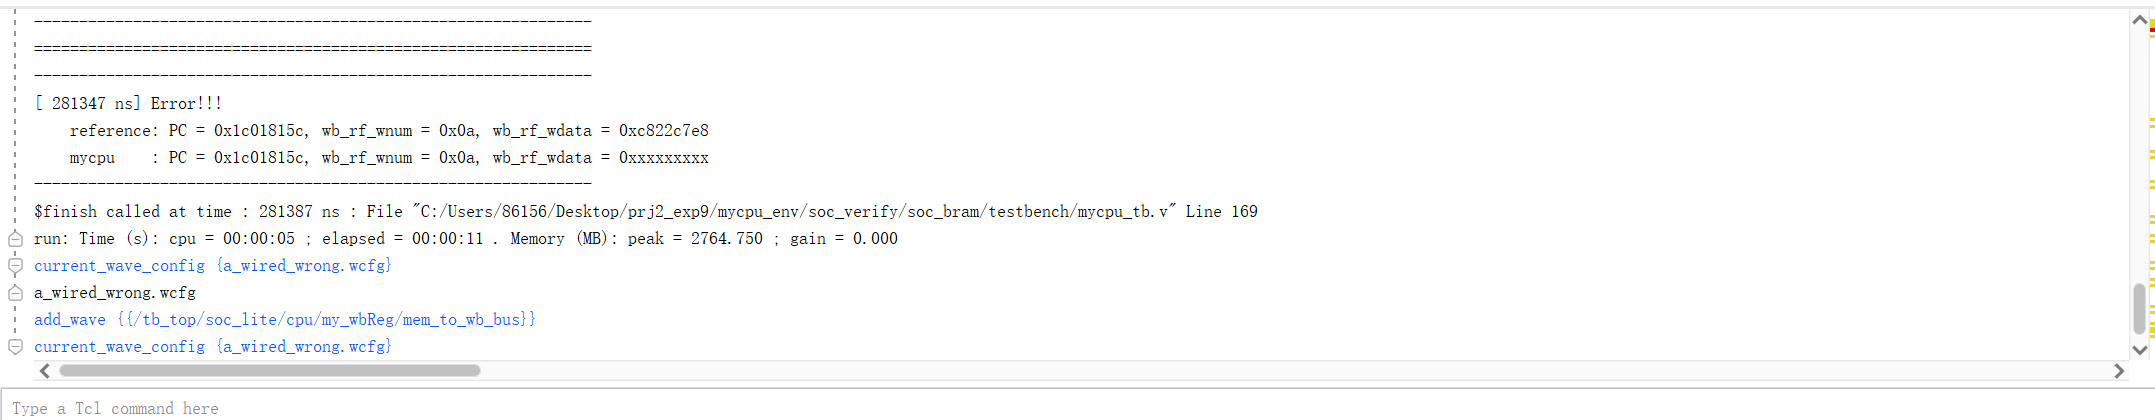
\includegraphics[width=10cm]{fig/2.png}
\end{figure}
\begin{figure}[H]
  \centering
  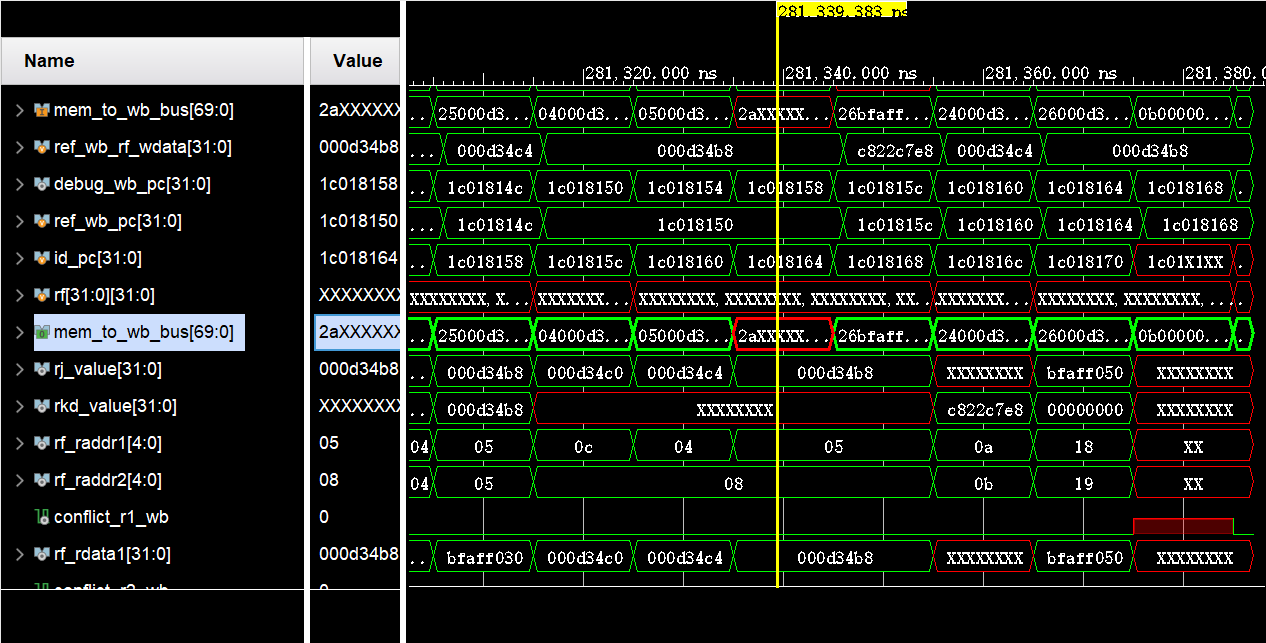
\includegraphics[width=10cm]{fig/3.png}
\end{figure}

分析可知,报错的地方来自于alu没有及时的返回乘法运算的结果,这是因为
alu乘法器需要两个周期进行运算,因此需要阻塞流水线进行等待。
添加在EX模块中的等待即可:
\begin{lstlisting}[language=verilog]
  assign ex_ready_go      = alu_complete;//等待alu完成运算
\end{lstlisting}

\end{document}